\section{Using Uintah} \label{Sec:UCF}

Several executable programs have been developed using the Uintah
Computational Framework (UCF).  The primary code that drives the
components implemented in Uintah is called \tt sus, \normalfont which
stands for Standalone Uintah Simulation.  The existing components were
originally developed to solve a complex fluid structure problem
involving a container filled with an explosive enveloped in a fire.

The code models the fire and the subsequent heat transfer to the
container followed by the resultant container deformation and ultimate
rupture due to the ignition and burning of the explosive material all
running on thousands of processors requiring thousands of hours of
computer time and hundreds of gigabytes of data storage.  Although
Uintah was developed originally to solve this complicated
multi-physics problem, the general nature of the algorithms and the
framework have allowed researchers to use the code to investigate a
wide range of problems.  The framework is general purpose enough to
allow for the implementation of a variety of implicit and explicit
algorithms on structured grids.  In addition, particle based
algorithms can be implemented using the native particle support found
in the framework.

This code leverages the task based parallelism inherent in the UCF to
implement several time stepping algorithms for structural mechanics,
fluid dynamics, and fluid structure interactions.  What follows is a
description of using \tt sus \normalfont within the realm of
structural mechanics, fluid mechanics, and structure-fluid
interactions.


%__________________________________
\subsection{Mechanics of Running sus}

For single processor simulations, the \tt sus \normalfont excutable
(Standalone Uintah Simulation) is run from the command line prompt
like this:
\begin{Verbatim}[fontsize=\footnotesize]
  sus input.ups
\end{Verbatim}
where \tt input.ups \normalfont is an xml formatted input file.  The
Uintah software release contains numerous example input files located
in the \tt src/StandAlone/inputs/UintahRelease \normalfont directory.

For multiprocessor runs, the user generally uses \tt mpirun
\normalfont to launch the code.  Depending on the environment, batch
scheduler, launch scripts, etc, \tt mpirun \normalfont may or may not
be used.  However, in general, something like the following is used:
\begin{Verbatim}[fontsize=\footnotesize]
  mpirun -np num_processors sus -mpi input.ups
\end{Verbatim}

\tt num\_processors \normalfont is the number of processors that will
be used.  The input file must contain a patch layout that has at least
the same number (or greater) of patches as processors specified by a
number following the -np option shown above.

In addition, the \tt -mpi \normalfont is optional but often times
necessary if the mpi environment is not automatically detected from
within the sus executable.

Uintah provides for restarting from checkpoint as well.  For information on
this, see Section~\ref{Sec:DataArchiver}, which describes how to create
checkpoint data, and how to restart from it.

\subsection{Uintah Problem Specification (UPS)} \label{Sec:UPS}

The Uintah framework uses XML like input files to specify the various
parameters required by simulation components.  These Uintah Problem
Specification (.ups) files are validated based on the specification
found in \tt src/StandAlone/inputs/UPS\_SPEC/ups\_spec.xml \normalfont
(and its sibling files).  

The application developer is free to use any of the specified tags to
specify the data needed by the simulation.  The essential tags that
are required by Uintah include the following:

\begin{Verbatim}[fontsize=\footnotesize]
  <Uintah_specification>

  <SimulationComponent>

  <Time>

  <DataArchiver>

  <Grid>
\end{Verbatim}


Individual components have additional tags that specify properties,
algorithms, materials, etc. that are unique to that individual
components.  Within the individual sections on MPM, ICE, MPMICE,
Arches, and MPMArches, the individual tags will be explained more
fully.

The sus executable verifies that the input file adheres to a consitent
specification and that all necessary tags are specified.  However, it
is up to the individual creating or modifying the input file to put in
physically reasonable set of consistent parameters.


\subsection{Simulation Components} \label{Sec:SimulationComponent}

The input file tag for SimulationComponent has the \tt type \normalfont
attribute that must be specified with either \tt mpm, mpmice, ice, arches,
\normalfont or \tt mpmarches, \normalfont as in:

\begin{Verbatim}[fontsize=\footnotesize]
<SimulationComponent type = "mpm" />
\end{Verbatim}



%__________________________________
\subsection{Time Related Variables} \label{Sec:TimeRelatedVariables}
Uintah components are time dependent codes.  As such, one of the first
entries in each input file describes the timestepping parameters.  An
input file segment is given below that encompasses all of the possible
parameters.  Most are self-explanatory, and not all are required, (e.g
\tt <max\_Timestep>, <max\_delt\_increase>,
<end\_on\_max\_time\_exactly> \normalfont and \tt <delt\_init>
\normalfont are all optional).  \tt <timestep\_multiplier> \normalfont
serves as a CFL number, that is, a number, usually less than 1.0, that
is used to moderate the timestep automatically calculated by the
individual components.

\begin{Verbatim}[fontsize=\footnotesize]
<Time>
    <maxTime>            1.0         </maxTime>
    <initTime>           0.0         </initTime>
    <delt_min>           0.0         </delt_min>
    <delt_max>           1.0         </delt_max>
    <delt_init>          1.0e-9      </delt_init>
    <max_delt_increase>  2.0         </max_delt_increase>
    <timestep_multiplier>1.0         </timestep_multiplier>
    <max_Timestep>       100         </max_Timestep>
    <end_on_max_time_exactly>true    </end_on_max_time_exactly>
</Time>
\end{Verbatim}
%
%__________________________________
\subsection{Data Archiver} \label{Sec:DataArchiver}

The Data Archiver section specifies the directory name where data will
be stored and what variables will be saved and how often data is saved
and how frequently the simulation is checkpointed.

The \tt <filebase> \normalfont tag is used to specify the directory
name and by convention, the \tt .uda \normalfont suffix is attached denoting the
``uintah data archive".

Data can be saved based on a frequency setting that is either based on time
intervals;\\
\tt <outputTimestepInterval> floating\_point\_time\_increment </outputTimestepInterval> \normalfont\\
or timestep intervals; \\
\tt <outputInterval> integer\_number\_of\_steps </outputInterval> \normalfont\\

Each simulation component specifies variables with label names that
can be specified for data output.  By convention, particle data is
denoted by \tt p. \normalfont followed by a particular variable name
such as mass, velocity, stress, etc.  Whereas for node based data, the
convention is to use the \tt g. \normalfont followed by the variable
name, such as mass, stress, velocity, etc.  Similarly, cell-centered
and face-centered data typically end with the a trailing \tt CC \normalfont
or \tt FC, \normalfont  respectively.  Within the DataArchiver
section, variables are specified with the following format:

\begin{Verbatim}[fontsize=\footnotesize]
   <save label = "p.mass" />
   <save label = "g.mass" />
\end{Verbatim}

To see a list of
variables available for saving for a given component, execute the following
command from the \tt StandAlone \normalfont directory:

\begin{Verbatim}[fontsize=\footnotesize]
inputs/labelNames component
\end{Verbatim}
where \tt component \normalfont is, e.g., \tt mpm, \normalfont \tt ice, \normalfont etc.

Checkpointing information can be created that provides a mechanism for
restarting a simulation at a later point in time.  The \tt
<checkpoint> \normalfont tag with the \tt cycle \normalfont and \tt
interval \normalfont attributes describe how many copies of checkpoint
data is stored (cycle)  and how often it is generated (interval).

As an example of checkpoint data that has two timesteps worth of
checkpoint data that is created every .01 seconds of simulation time
is shown below:

\begin{Verbatim}[fontsize=\footnotesize]
<checkpoint cycle = "2" interval = "0.01"/>
\end{Verbatim}


To restart from a checkpointed archive, simply put "-restart" in the
sus command-line arguments and specify the .uda directory instead of
a ups file (sus reads the copied \tt input.xml \normalfont from the
archive).  One can optionally specify a certain timestep to restart
from with \tt -t timestep \normalfont with multiple checkpoints, but the
last checkpointed timestep is the default.  When restarting, sus
copies all of the appropriate information from the old uda directory to its
new uda directory.
% I'M NOT SURE ABOUT THIS, -nocopy REMOVES THE OLD UDA?  I THOUGHT IT
% JUST LEFT STUFF IN THE OLD UDA, WHERE AS -copy MADE A COPY OF OLD TIMESTEP
% DATA, AND -move MOVED THE OLD TIMESTEP DATA TO THE NEW UDA.  
%  If one doesn't want to keep the old uda directory
%around, they can specify \tt -nocopy \normalfont to have it be removed
%(e.g., if you are cramped for disk space).  Either way it creates a new uda
%directory for you as always.

Here are some example:

\begin{Verbatim}[fontsize=\footnotesize]
./sus -mpm -restart disks.uda.000 -nocopy
./sus -mpm -restart disks.uda.000 -t 29
\end{Verbatim}
%
%__________________________________
\subsection{Geometry objects} \label{Sec:GeometryObjects}
%FIXME
%- what is res \\

Within several of the components, the material is described by a
combination of physical parameters and the geometry.  Geometry objects
use the notion of constructive solid geometry operations to compose
the layout of the material from simple shapes such as boxes, spheres,
cylinders, as well as operators which include the union,
intersections, differences of the simple shapes.  In addition to the
simple shapes, triangulated surfaces can be used in conjunction with
the simple shapes and the operations on these shapes.

Each geometry object has the following properties, label (string
name), type (box, cylinder, sphere, etc), resolution (vector
quantity), and any unique geometry parameters such as origin, corners,
triangulated data file, etc.  The operators which include, the union,
the difference, and intersection tags contain either lists of
additional operators or the primitives pieces.

As an example of a non-trivial geometry object is shown below:

\begin{Verbatim}[fontsize=\footnotesize]
<geom_object>

     <intersection>
       <box label = "Domain">
          <min>[0.0,0.0,0.0]</min>
          <max>[0.1,0.1,0.1]</max>
       </box>
       <union>
         <sphere label = "First node">
            <origin>[0.022,0.028,0.1  ]</origin>
            <radius>0.01</radius>
         </sphere>
         <sphere label = "2nd node">
            <origin>[0.030,0.075,0.1  ]</origin>
            <radius>0.01</radius>
         </sphere>
       </union>
     </intersection>
     <res>[2,2,2]</res>
     <velocity>[0.,0.,0.]</velocity>
     <temperature>0 </temperature>
</geom_object>
\end{Verbatim}

The following geometry objects are given with their required tags:

\tt box \normalfont has the following tags: min and max which are vector quantities
specified in the \tt [a, b, c] \normalfont format.

\tt sphere \normalfont has an origin tag specified as a vector and the radius tag
specified as a float.

\tt cone \normalfont has a tag for the top and bottom origins (vector) as well as tags for the
top and bottom radius (float) to create a right circular cone/frustram.

\tt cylinder \normalfont has a tag for the top and bottom origins (vector) plus a tag
for the radius (float).

\tt sphere \normalfont has a tag for the origin (vector) and the radius (float).

\tt tri \normalfont is a tag for describing a triangulated surface.  The name tag
specifies the file name to use for reading in the triangulated surface
description and the points file.  The triangulated surface
(file\_name.tri) contains a list of integers describing the
connectivities of points specified in file\_name.pts.  Here is an
excerpt from a tri file and a points file:


\begin{Verbatim}[fontsize=\footnotesize]
Triangulated file

1 39 41
1 41 38
38 41 42
. . .

Points file

0 0.03863 -0.005
0.35227 0.13023 -0.005
0.00403479 0.0296797 -0.005
. . .

\end{Verbatim}

The boolean operators on the geometry pieces include \tt difference, intersection, \normalfont and \tt union.\normalfont 

The \tt difference  \normalfont takes two geometry pieces and subtracts the second
geometry piece from the first geometry piece.  The \tt intersection \normalfont
operator requires at least two geometry pieces in forming an
intersection geometry piece.  Whereas the \tt union \normalfont operator aggregates a
collection of geometry pieces.  Multiple operators can be used to form
very complex geometry pieces.


%__________________________________
\subsection{Boundary conditions}

Boundary conditions are specified within the \tt <Grid> \normalfont
but are described separately for clarity.  The essential idea is that
boundary conditions are specified on the domain of the grid.  Values
can be assigned either on the entire face, or parts of the face.
Combinations of various geometric descriptions are used to aid in the
assignment of values over specific regions of the grid.  Each of the
six faces of the grid is denoted by either the minus or plus side of
the domain.

The xml description of a particular boundary condition includes which
side of the domain, the material id, what type of boundary condition
(Dirichlet or Neumann) and which variable and the value assigned.  The
following is a an MPM specification of a Dirichlet boundary condition
assigned to the velocity component on the x minus face (the entire
side) with a vector value of [0.0,0.0,0.0] applied to all of the materials.

\begin{Verbatim}[fontsize=\footnotesize]

 <Grid>
       <BoundaryConditions>
         <Face side = "x-">
             <BCType id = "all" var = "Dirichlet" label = "Velocity">
                   <value> [0.0,0.0,0.0] </value>
             </BCType>
         </Face>
         <Face side = "x+">
            <BCType id = "all" var = "Dirichlet" label = "Velocity">
                 <value> [0.0,0.0,0.0] </value>
            </BCType>
         </Face>
        . . . .
        <BoundaryCondition>
   . . . .
  <Grid>

\end{Verbatim}

The notation \tt <Face side = "x-"> \normalfont indicates that the
entire x minus face of the boundary will have the boundary condition
applied.  The \tt id = "all" \normalfont means that all the
materials will have this value.  To specify the boundary condition for
a particular material, specify an integer number instead of the
"all".  The \tt var = "Dirichlet" \normalfont is used to specify
whether it is a Dirichlet or Neumann or symmetry boundary conditions.
Different components may use the \tt var \normalfont to include a
variety of different boundary conditions and are explained more fully
in the following component sections.  The \tt label = "Velocity"
\normalfont specifies which variable is being assigned and again is
component dependent.  The \tt <value> [0.0,0.0,0.0] </value>
\normalfont specifies the value.

An example of a more complicated boundary condition demonstrating a
hot jet of fluid issued into the domain is described.  The jet is
described by a circle on one side of the domain with boundary
conditions that are different in the circular jet compared to the rest
of the side.

\begin{Verbatim}[fontsize=\footnotesize]

 <Face circle = "y-" origin = "0.0 0.0 0.0" radius = ".5">
        <BCType id = "0"   label = "Pressure" var = "Neumann">
                              <value> 0.0   </value>
        </BCType>
        <BCType id = "0" label = "Velocity" var = "Dirichlet">
                              <value> [0.,1.,0.] </value>
        </BCType>
        <BCType id = "0" label = "Temperature" var = "Dirichlet">
                              <value> 1000.0  </value>
        </BCType>
        <BCType id = "0" label = "Density" var = "Dirichlet">
                              <value> .35379  </value>
        </BCType>
        <BCType id = "0" label = "SpecificVol"  var = "computeFromDensity">
                              <value> 0.0  </value>
        </BCType>
      </Face>
      <Face side = "y-">
        <BCType id = "0"   label = "Pressure"     var = "Neumann">
                              <value> 0.0   </value>
        </BCType>
        <BCType id = "0" label = "Velocity"     var = "Dirichlet">
                              <value> [0.,0.,0.] </value>
        </BCType>
        <BCType id = "0" label = "Temperature"  var = "Neumann">
                              <value> 0.0  </value>
        </BCType>
        <BCType id = "0" label = "Density"      var = "Neumann">
                              <value> 0.0  </value>
        </BCType>
        <BCType id = "0" label = "SpecificVol"  var = "computeFromDensity">
                              <value> 0.0  </value>
        </BCType>
      </Face>

\end{Verbatim}

The jet is described by the circle on the y minus face with the origin
at 0,0,0 and a radius of .5.  For the region outside of the circle,
the boundary conditions are different.  Each side must have at least
the \tt "side" \normalfont specified, but additional circles and
rectangles can be specified on a given face.

An example of the \tt rectangle \normalfont is specified as with the
lower corner at 0,0.181,0 and upper corner at 0,0.5,0.


\begin{Verbatim}[fontsize=\footnotesize]
 <Face rectangle = "x-" lower = "0.0 0.181 0.0" upper = "0.0 0.5 0.0">
\end{Verbatim}

%
%__________________________________
\subsection{Grid specification} \label{Sec:Grid}

The \tt <Grid> \normalfont section specifies the domain of the
structured grid and includes tags which indicate the lower and upper
corners, the number of extra cells which can be used by various
components for the application of boundary conditions or interpolation
schemes.  

The grid is decomposed into a number of patches.  For single processor
problems, usually one patch is used for the entire domain.  For
multiple processor simulations, there must be at least one patch per
processor.  Patches are specified along the x,y,z directions of the
grid using the \tt <patches> [2,5,3] </patches> \normalfont which
specifies two patches along the x direction, five patches along the y
direction and 3 patches along the z direction.  The maximum number of
processors that \tt sus \normalfont could use is $2X5X3 = 30$.
Attempting to use more processors than patches
will cause a run time error during initialization.

Finally, the grid spacing can specified using either a fixed number of
cells along each x,y,z direction or by the size of the grid cell in
each direction.  To specify a fixed number of grid cells, use the \tt
<resolution> [20,20,3] </resolution> \normalfont.  This specifies 20
grid cells in the x direction, 20 in the y direction and 3 in the z
direction.  To specify the grid cell size use the \tt <spacing>
[0.5,0.5,0.3] </spacing> \normalfont.  This specifies the a grid cell
size of .5 in the x and y directions and .3 in the z direction.  The
\tt <resolution> \normalfont and \tt <spacing> \normalfont cannot be
specified together.  The following two examples would generate
identical grids:

\begin{Verbatim}[fontsize=\footnotesize]
<Level>
    <Box label="1">
       <lower>        [0,0,0]          </lower>
       <upper>        [5,5,5]          </upper>
       <extraCells>   [1,1,1]          </extraCells>
       <patches>      [1,1,1]          </patches>
    </Box>
    <spacing>         [0.5,0.5,0.5]    </spacing>
</Level>
\end{Verbatim}
\begin{Verbatim}[fontsize=\footnotesize]
<Level>
    <Box label="1">
       <lower>        [0,0,0]          </lower>
       <upper>        [5,5,5]          </upper>
       <resolution>   [10,10,10]       </resolution>
       <extraCells>   [1,1,1]          </extraCells>
       <patches>      [1,1,1]          </patches>
    </Box>
</Level>
\end{Verbatim}


The above examples indicate that the grid domain has a lower corner at
0,0,0 and an upper corner at 5,5,5 with one extra cell in each
direction.  The domain is broken down into one patch covering the
entire domain with a grid spacing of .5,.5,.5.  Along each dimension
there are ten cells in the interior of the grid and one layer of
``extraCells" outside of the domain.  extraCells are the Uintah nomenclature
for what are frequently referred to as ``ghost-cells".

%
%__________________________________
\subsection{Adapative Mesh Refinement}
- Describe refinement flags
- Describe boundary layers
- How is a cell flagged as needing to be refined
%
%__________________________________
\subsection{Regridder}

The regridder creates a multilevel grid from the refinement flags.
Each level will completely cover the refinement flags from the corser
level.  The primary regridder used in Uintah is the \emph{Tiled} regridder.
The tiled regridder creates a set of evenly sized tiles across the domain
that will become patches if refinement is required in the tiles region.

The following is an example of this regridder.

\begin{Verbatim}     
<Regridder type="Tiled">   
    <max_levels>2</max_levels>
    <cell_refinement_ratio> [[2,2,1]] </cell_refinement_ratio>
    <cell_stability_dilation> [2,2,0] </cell_stability_dilation>
    <min_boundary_cells> [1,1,0] </min_boundary_cells>
    <min_patch_size>  [[8,8,1]] </min_patch_size>
    <dynamic_size> true </dynamic_size>      
    <patches_per_level_per_proc>8</patches_per_level_per_proc>   
</Regridder>
\end{Verbatim}

The \emph{max\_levels} tag specifies the maximum number of levels
to be created.  The \emph{cell\_refinement\_ratio} tag specifies the 
refinement ratio between the levels.  This can be specified on a per 
level basis as follows:

\begin{Verbatim}
    <cell_refinement_ratio> [[2,2,1],[4,4,1]] </cell_refinement_ratio>
\end{Verbatim}

The \emph{cell\_stability\_dilation} tag specifies how many cells around
the refinement flags are also gaurenteed to be refined.  The
\emph{min\_boundary\_cells} tag specifies the size of the boundary layers. 
The size of the tiles is specified using the \emph{min\_patch\_size} tag
and can also be specified on a per level basis.

Finally the size of the tiles can change at run time.  If the number
of patches is higher than what is needed then the tile size will double in
the smallest dimension.  Conversely if the target number of patches is low
then the tile size will halve in the longest dimension but will never go
below the \emph{min\_patch\_size}.  The target number of patches per processor is 
specified using the \emph{patches\_per\_level\_per\_proc} tag. To prevent the 
resizing of tiles set the tag \emph{dynamic\_size} to false. 

%
%__________________________________
\subsection{Load Balancer}

The load balancer assignes patches to processors such that work is 
evenly distributed.  Uintah currently supports a wide array of 
load balancing algorithms.  To specify a load balancing algorithm 
add a block similar to the following:

\begin{Verbatim}
  <LoadBalancer type="DLB">
       <dynamicAlgorithm>patchFactor</dynamicAlgorithm>
       <timestepInterval>50</timestepInterval>
       <gainThreshold>0.05</gainThreshold>
  </LoadBalancer>
\end{Verbatim}

The type specifies which load balancer is used.  The type can be \emph{DLB}, 
\emph{RoundRobin}, \emph{SimpleLoadBalancer}, or \emph{SingleProcessorLoadBalancer}.  
If no load balancer is specified than either the SimpleLoadBalancer 
or the SingleProcessorLoadBalancer will be used.  For complex problems including 
AMR the DLB load  balancer should be used.  This load balancer uses advanced 
algorithms to achieve more efficient patch assignments.  To use the DLB load 
balancer you must include the  \emph{dynamicAlgorithm} tag. This tag can be 
\emph{PatchFactor} or \emph{Zoltan}.  

\begin{Verbatim}
       <dynamicAlgorithm>patchFactor</dynamicAlgorithm>
\end{Verbatim}

Both of these algorithms compute the weight of a patch using either a profiling model 
or an algorithm cost model.  By default  the profiling model is used as it provides 
highly accurate estimates and does not require the specification of model parameters.  
To disable profiling add the tag

\begin{Verbatim}
       <doCostProfiling>false</doCostProfiling>
\end{Verbatim}

This will cause the load balancer to use the cost model $W_p=N_pc_1+N_cc_2+c_3$ to 
determine the weight of a patch, where $N_p$ is the number of particles 
in the patch, $N_c$ is the number of cells on the patch, $c_1$ is the weight per
particle, $c_2$ is the weight per cell, and $c_3$ is a constanct cost on the
patch.  These constants can be specified with the following tags:

\begin{Verbatim}
       <cellCost>1</cellCost>
       <particleCost>1.25</particleCost>
       <patchCost>4</patchCost>
\end{Verbatim}

The number of particles will always be zero unless the algorithm is instructed to
collect particles with the collectParticles tag.  

\begin{Verbatim}
       <collectParticles>true</collectParticles>
\end{Verbatim}

The following are a couple of extra load balancer parameters that may be useful.
\begin{Verbatim}
       <timestepInterval>50</timestepInterval>
       <gainThreshold>0.05</gainThreshold>
       <outputNthProc>8</outputNthProc>
\end{Verbatim}

The \emph{timestepInterval} tag specifies the maximum number of timesteps the simulation
can run without attempting to load balance.  The \emph{gainThreshold} tag specifies the 
percent improvement that a load balance must provide over the old load balance in 
order for the new load balance to be used.  Finally the \emph{outputNthProc} tag causes
the data archive to be written to by every Nth processor instead of every processor.  
This can allieviate problems caused by having to many processors attempting to write 
to the same file system at the same time. 

If the dynamic algorithm is set to \emph{Zoltan} then the user must also specify which
Zoltan algorithm to use with the \emph{zoltanAlgorithm} tag.  

\begin{Verbatim}
       <zoltanAlgorithm>HSFC</zoltanAlgorithm>
\end{Verbatim}

The Zoltan algorithm can be set to \emph{HSFC}, \emph{RIB}, \emph{RCB}.

%__________________________________
\subsection{UDA}

\subsubsection{UDA Directory Structure}

The UDA is a file/directory structure used to save Uintah simulation
data.  For the most part, the user need not concern him or herself
with the UDA layout, but it is a good idea to have a general feeling
for how the data is stored on disk...

%\subsubsubsection{UDA Naming}

Every time a simulation (sus) is run, a new UDA is created.  Sus uses
the <filebase> tag in the simulation input
(FIXME: link to [[Documentation/UsersGuide Input\_Files|.ups]]) file to name the UDA
directory (appending a version number).  If an UDA of that name
already exists, the next version number is used.  Additionally, a
symbolic link named ``disks.uda'' (is updated to and) will point to
the newest version of this simulations UDA.  Eg:

disks.uda.000
disks.uda.001
disks.uda.001 <- disks.uda

%\subsubsubsection{UDA Files}

Each UDA consists of a number of top level files, a checkpoints
subdirectory, and subdirectories for each saved timestep.  These files
include:

- \tt.dat\normalfont files contain global information about the simulation
(each line in the .dat files contains: simulation\_time value).
- The \tt checkpoints\normalfont directory contains a limited number of time
step data subdirectories that contain a complete snapshot of the
simulation (allowing for the simulation to be restarted from that
time).
- \tt input.xml\normalfont contains the original problem specification (the
.ups file).
- \tt index.xml\normalfont contains information on the actual simulation run.
- \tt t0000 FIXME number sign\normalfont contains data saved for that specific time step.  The
data saved is specified in .ups file and may be a very limited subset
of the full simulation data.

Example UDA file list:

CenterOfMassPosition.dat
CenterOfMassVelocity.dat
KineticEnergy.dat
StrainEnergy.dat
TotalMass.dat
checkpoints
index.xml
input.xml
t00001
t00057

%\subsubsection{Known Issues}

Occasionally, due (most likely) to file system issues on large
clusters, some of the files in the UDA have been found to be corrupted
or nonexistent.  (There is error checking in the code to try to
prevent this.  We believe that either the OS/File system is
incorreclty returning error codes, or, more likely, that the files are
corrupted (due to file system issues) after the simulation is done.

%\subsubsection{Restarting}

The sus executable provides a mechanism for checkpointing the code and
then restarting the ongoing simulation from a given checkpoint.



%__________________________________
\subsection{Visualization tools}

Visualization of Uintah data is currently possible using any of three
software packages.  These are SCIRun, VisIt and Manta.  Of these, SCIRun is
no longer supported, although legacy versions will continue to work.  The
VisIt package from LLNL is general purpose visualization software that offers
all of the usual capabilities for rendering scientific data.  It is still
developed and maintained by LLNL staff, and its interface to Uintah data is
supported by the Uintah team.  Manta offers volume rendering and particle
visualizaton based on parallel (shared memory) ray tracing techniques.
While the capabilities of Manta are more limited, it is a fast way to
interactively interrogate reasonably large datasets, provided the user has
access to a reasonable shared memory resource, (e.g. an 8 core desktop system).

\subsubsection{VisIt}

\paragraph{Reading Uintah Data Archive's}

Once you have installed VisIt and the UDA reader plugin, you can launch VisIt and start visualizing UDA's. To open a UDA, select \tt Open File \normalfont from the \tt  File \normalfont menu. Browse into the UDA you want to load and select the \tt index.xml \normalfont file. Then hit on \tt OK \normalfont and a list of timesteps should now appear on the gui. Figure~\ref{VisItFileOpen} illustrates this process.

\begin{figure}
  \center
  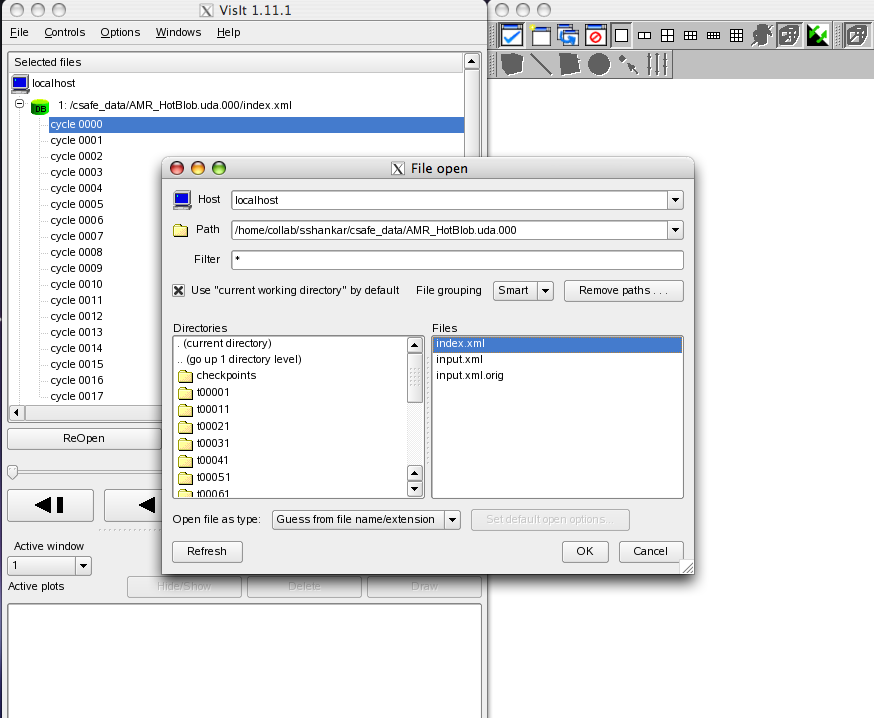
\includegraphics[scale=0.5]{VisItFileOpen.png}
  \caption{Opening an UDA with VisIt}
  \label{VisItFileOpen}
\end{figure}

\paragraph{Plots}

VisIt displays data as plots. A plot might render a specific variable or it might render the structure of the mesh. Figure~\ref{VisItPlots} illustrates this.

\begin{figure}
  \center
  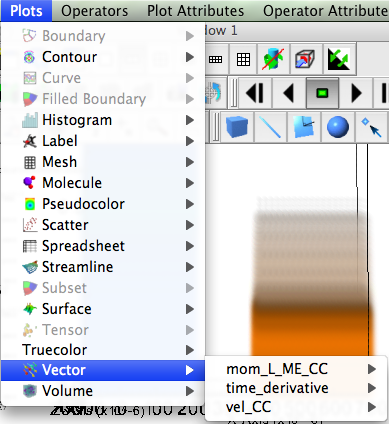
\includegraphics[scale=0.75]{VisItPlots.png}
  \caption{Various plots in VisIt}
  \label{VisItPlots}
\end{figure}

Note that VisIt attempts to analyze the variables and associate them with the appropriate plots. As shown in figure~\ref{VisItPlots}, only vector variables are available for the vector plot. The most commonly used plots for visualizing UDA's are Pseudocolor, Volume and the Vector plot. The Subset plot can be used to visualize the structure of patches in an AMR dataset. %The Mesh plot can be used to display the mesh structure.

Once you have a plot, you change plot attributes by clicking on the PlotAtts menu and selecting the plot of you choice. Alternatively, you may double click on the plot itself in Active plots window. For example, if you have a Volume plot and you want to change its attributes, the window shown in figure~\ref{VisItVolumeAtts} pops up.

\begin{figure}
  \center
  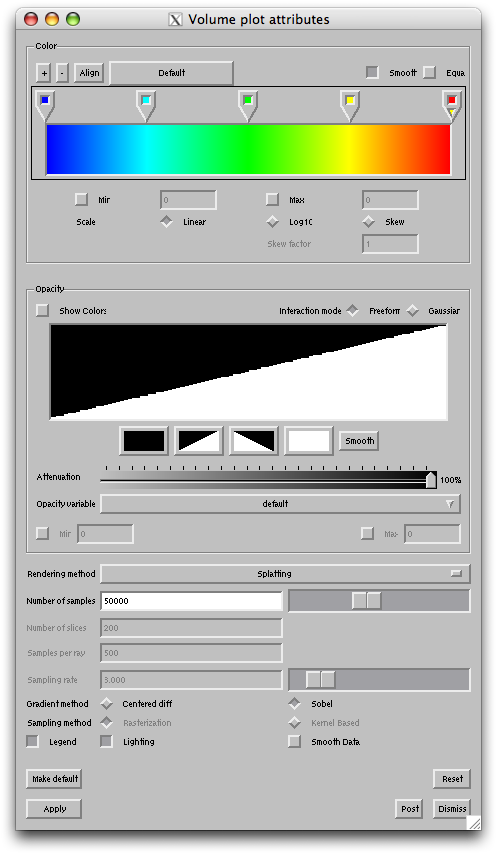
\includegraphics[scale=0.65]{VisItVolumeAtts.png}
  \caption{Volume plot attributes in VisIt}
  \label{VisItVolumeAtts}
\end{figure}

As seen in figure~\ref{VisItVolumeAtts}, you can change the color map, opacity curve, rendering method, no. of samples, lighting options, etc. in this window.

\paragraph{Operators}

A wide variety of operators can be applied to the plots, as mentioned earlier. These modify the incoming datasets in some way (eg., a slice formats a 3D dataset into a 2D slice), which can then be plotted. However, you will first need to select a plot and then only you can apply an operator to it (though the order of operation is opposite). An important thing to keep in mind is that when you select an operator, by default it gets applied to all the plots in the Active plots window. You will need to uncheck the Apply operators checkbox, in case you just want to apply the operator to a single plot. This is illustrated in figure~\ref{VisItApplyOperators}.

\begin{figure}
  \center
  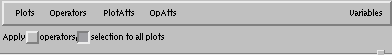
\includegraphics[scale=0.75]{VisItApplyOperators.png}
  \caption{Unchecking "selection to all plots"}
  \label{VisItApplyOperators}
\end{figure}

The entire list of operators that VisIt supports can be seen by clicking on the Operators menu. Also, once you have applied an operator, you can change its attributes by clicking on the OpAtts menu and then clicking on the desired operator.
Figures~\ref{VisItSelectPlot} and~\ref{VisItSelectOperator} illustrate how you can apply a Slice operator to a Pseudocolor plot and then change the operator attributes.
First, apply the Pseudocolor plot to a desired variable, and then select the Slice operator from the Operators menu.

\begin{figure}
  \center
  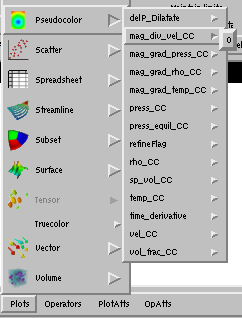
\includegraphics[scale=0.75]{VisItSelectPlot.png}
  \caption{Applying the Pseudocolor plot to a variable}
  \label{VisItSelectPlot}
\end{figure}

\begin{figure}
  \center
  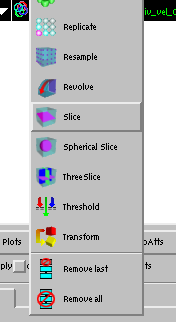
\includegraphics[scale=0.75]{VisItSelectOperator.png}
  \caption{Applying an operator to a plot}
  \label{VisItSelectOperator}
\end{figure}

At this point in time, you should have an ordering similar to that in figure~\ref{VisItOrderOperator}.  

\begin{figure}
  \center
  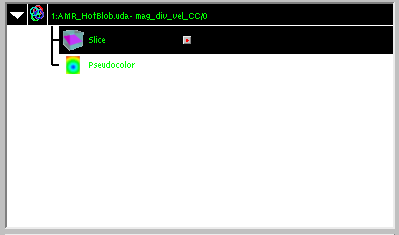
\includegraphics[scale=0.75]{VisItOrderOperator.png}
  \caption{Ordering of an operator and a plot}
  \label{VisItOrderOperator}
\end{figure}

Once you have this order, select Slice from the OpAtts menu. This will pop up the Slice operator attributes window, as shown in figure~\ref{VisItSliceAtts}.

\begin{figure}
  \center
  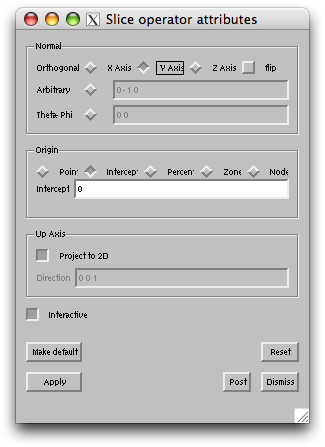
\includegraphics[scale=0.75]{VisItSliceAtts.png}
  \caption{Slice plot attributes in VisIt}
  \label{VisItSliceAtts}
\end{figure}

You can now play up with the various attributes (eg., selecting normal plane) to obtain the desired visualization. The checkbox "Project to 2D" should be unchecked is you want to have the slice in 3D space.

\paragraph{Vectors}

By default, VisIt reduces the number of vectors plotted (to 400) and this needs to be manually changed to the original number or something greater, only if required.
This can be accomplished by changing the attributes of the Vector plot. In figure~\ref{VisItVectorNumber}, the no of vectors has been increased to 2000.

\begin{figure}
  \center
  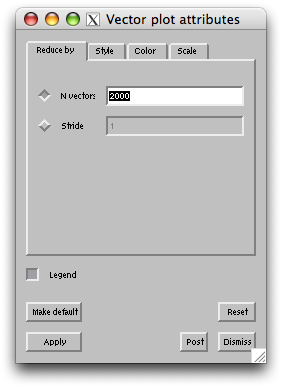
\includegraphics[scale=0.75]{VisItVectorNumber.png}
  \caption{Increasing the number of Vectors}
  \label{VisItVectorNumber}
\end{figure}

Also if you would like all the vectors to be visible, you would need to switch off both the options,
\tt Scale by magnitude
\normalfont and
\tt Auto scale
\normalfont under the Scale tab in the same window.

Figure~\ref{VisItVectorScale} describes this.

\begin{figure}
  \center
  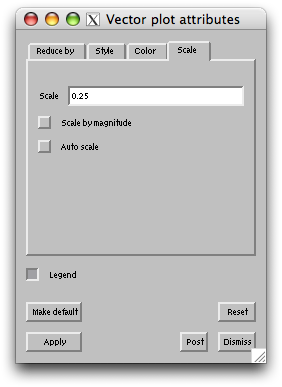
\includegraphics[scale=0.75]{VisItVectorScale.png}
  \caption{Increasing the number of Vectors}
  \label{VisItVectorScale}
\end{figure}

\paragraph{AMR datasets}

AMR datasets are read the same way as single level datasets. Once you have it read, you can apply an plot/ operator on it. Since the dataset is organized as levels and patches, you now have the flexibility of visualizing each of them independently or as in a group. To achieve this (assuming that you have already selected a plot), click on the Subset button either on the Active Plots window in the gui or on the same option in the Controls menu. This is illustrated in figures~\ref{VisItSubsetIcon} and ~\ref{VisItSubsetWin}.

\begin{figure}
  \center
  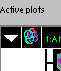
\includegraphics[scale=1.0]{VisItSubsetIcon.png}
  \caption{Clicking on this icon pops up the Subset window}
  \label{VisItSubsetIcon}
\end{figure}

\begin{figure}
  \center
  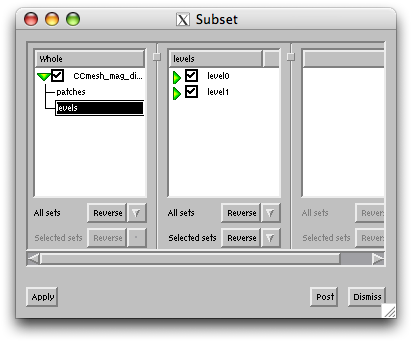
\includegraphics[scale=0.75]{VisItSubsetWin.png}
  \caption{The Subset window in VisIt}
  \label{VisItSubsetWin}
\end{figure}

\paragraph{Examples}

\subparagraph{Volume visualization}

a. Read in the uda by selecting the index.xml file. A list of timesteps should now appear on the gui.

b. The first timestep (cycle 0000) should be preselected. In case you are interested in plotting a different timestep, just double click on it. Alternatively you can type it in the small rectangular box (figure~\ref{VisItTimestepBox}), just below the list of timesteps. This can also be done at a later period in time, when you are done plotting the variable associated with a specific timestep and want to traverse through the others.

\begin{figure}
  \center
  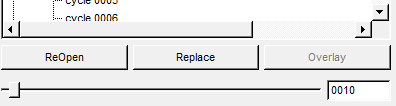
\includegraphics[scale=0.75]{VisItTimestepBox.png}
  \caption{The window on the gui lists all the timesteps}
  \label{VisItTimestepBox}
\end{figure}

c. Next we select a variable to plotted. We click on the Plots menu, select the Volume plot and then select the variable tempIN as shown in the figure~\ref{VisItVolumeTempINATK08}. The number '1' refers to the material associated with the variable.

\begin{figure}
  \center
  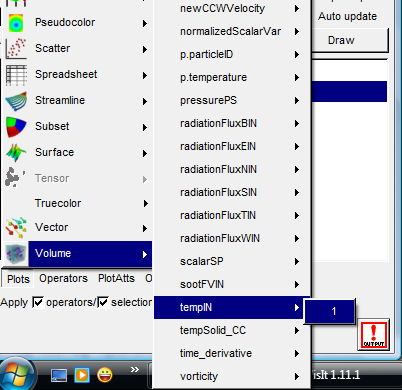
\includegraphics[scale=0.75]{VisItVolumeTempINATK08.png}
  \caption{Selecting a volume plot and an associated variable/ material}
  \label{VisItVolumeTempINATK08}
\end{figure}

d. The variable tempIN/1 now appears on the Active plots window (figure~\ref{VisItDrawTempINATK08}). Select the variable and click Draw.

\begin{figure}
  \center
  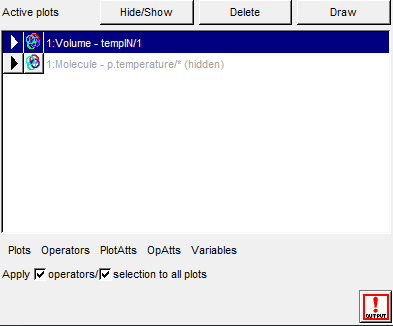
\includegraphics[scale=0.75]{VisItDrawTempINATK08.png}
  \caption{The list of plots in the Active plots window}
  \label{VisItDrawTempINATK08}
\end{figure}

e. A visualization now appears on the Viewer window, as shown in figure~\ref{VisItVolumeTempINATK08Viewer}. You can interact with the visualization in terms of rotating it (holding the left mouse button and dragging it), zooming in/ out (scrolling the roller on the mouse and/ or selecting the magnifier at the top of the Viewer window) etc.

\begin{figure}
  \center
  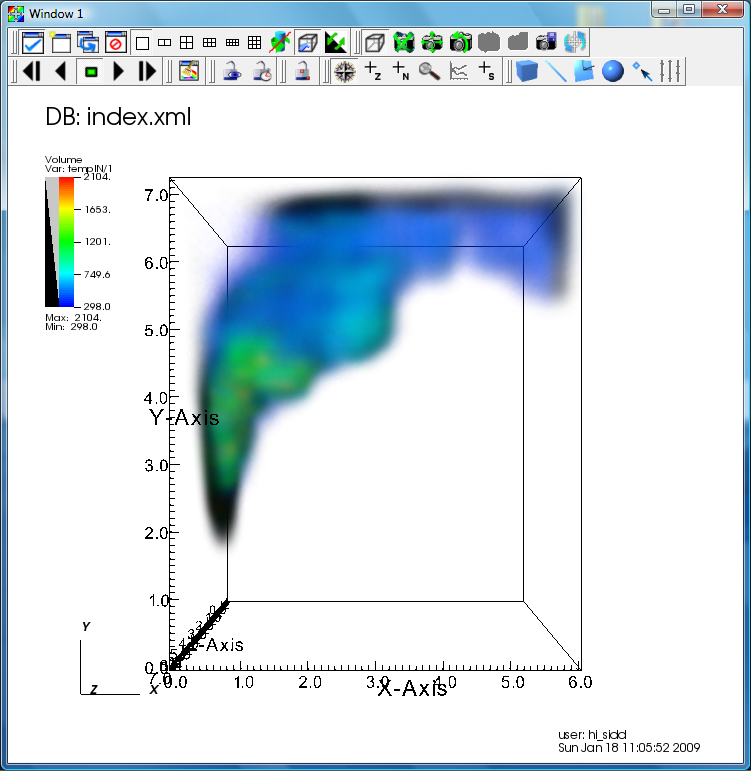
\includegraphics[scale=0.5]{VisItVolumeTempINATK08Viewer.png}
  \caption{Visualization of a volume on the viewer window}
  \label{VisItVolumeTempINATK08Viewer}
\end{figure}

f. Once you have this basic volume visualization, you can change its attributes by double clicking on the Volume - tempIN/1 plot in the Active plots window. This pops up the Volume plot attributes window (figure~\ref{VisItVolumeAttributes1} and figure~\ref{VisItVolumeAttributes2}).

\begin{figure}
  \center
  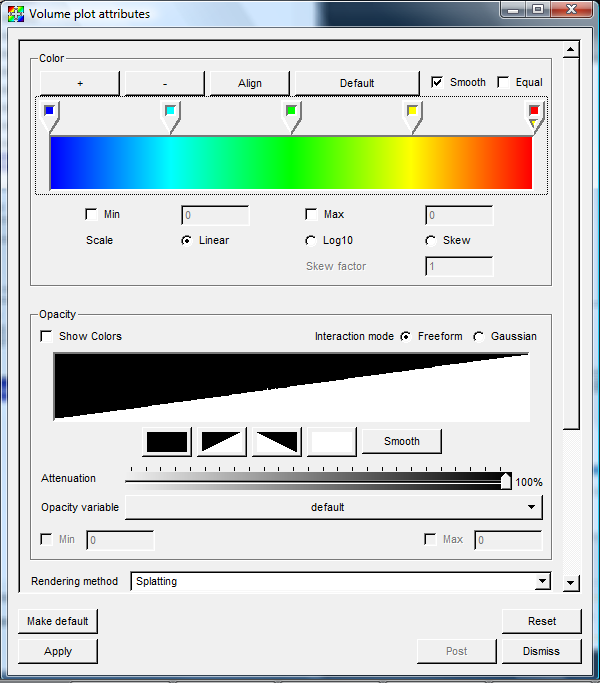
\includegraphics[scale=0.5]{VisItVolumeAttributes1.png}
  \caption{Volume visualization attributes window}
  \label{VisItVolumeAttributes1}
\end{figure}

\begin{figure}
  \center
  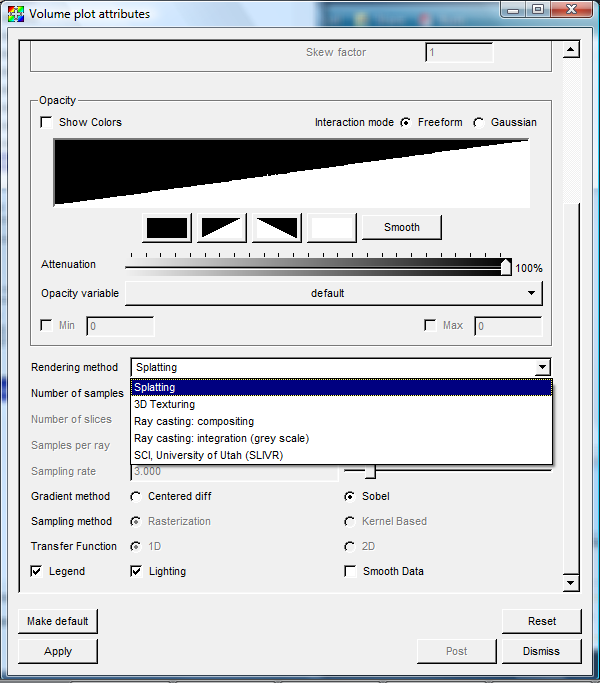
\includegraphics[scale=0.5]{VisItVolumeAttributes2.png}
  \caption{Volume visualization attributes window}
  \label{VisItVolumeAttributes2}
\end{figure}

The tab Color specifies the color table and the various options associated with it. The user can add/ remove control points by clicking on the + and - buttons. These can then be equally spaced by pressing the Align button.

A different color table can be selected by clicking on the Default button and then selecting an appropriate color table. The color(s) associated with the control points can be changed by right-clicking on the them and then selecting an appropriate color.

The user also has the option of specifying a Min and Max on the scalar value range by checking on the associated box(s) and entering in the values.

The second tab Opacity lets you specify a transfer function for the color table. Clicking on the check box Show Colors copies the colors from the color table onto this graph. Selecting the Interaction Mode as Gaussian lets you draw curves and specify a more accurate color table (figure~\ref{VisItTransferFunction}).

\begin{figure}
  \center
  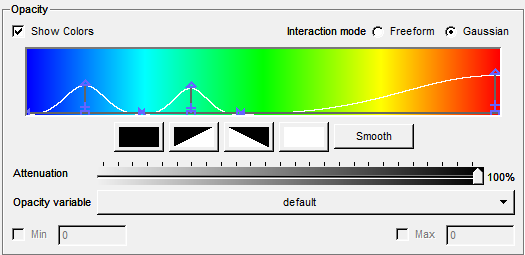
\includegraphics[scale=0.75]{VisItTransferFunction.png}
  \caption{The opacity trasfer function in the attributes window}
  \label{VisItTransferFunction}
\end{figure}

You can add in as many curves on the graph by clicking on the left mouse button and then placing them accordingly. To delete an unwanted curve, just right click on it.

After specifying an opacity transfer function, one can select an appropriate rendering method, Splatting being the default. The related fields thereafter become active/ inactive as and when different rendering methods are selected.

\subparagraph{Particles}

a. To add particles, we select the Molecule plot and then click on the variable p.temperature as shown in the figure~\ref{VisItMoleculePTempATK08}. The asterisk '*' refers to all the materials associated with the variable.

\begin{figure}
  \center
  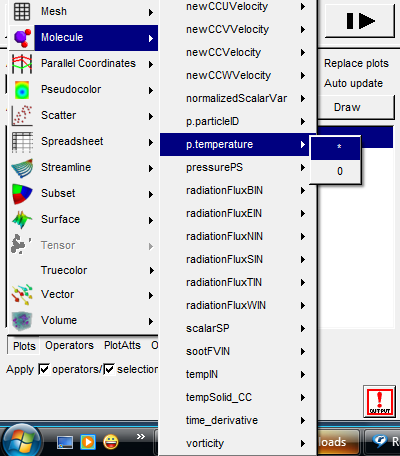
\includegraphics[scale=0.75]{VisItMoleculePTempATK08.png}
  \caption{Selecting a molecule plot and an associated variable/ material}
  \label{VisItMoleculePTempATK08}
\end{figure}

b. The variable p.temperature/* now appears on the Active plots list. Select the variable and hit Draw. A container in the form of particles now appears on the Viewer window.

c. Now double click on the variable name in Active plots list. This brings up the Molecule plot attributes window as shown in figure~\ref{VisItMoleculeAttributesPTemp1}.

\begin{figure}
  \center
  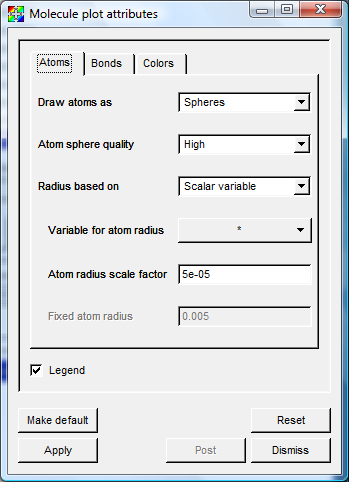
\includegraphics[scale=0.75]{VisItMoleculeAttributesPTemp1.png}
  \caption{Selecting a molecule plot and an associated variable/ material}
  \label{VisItMoleculeAttributesPTemp1}
\end{figure}

We choose to visualize the particles as Sphere Imposters (doesn't runs the GPU out of memory, drawing as Spheres does). We also choose to scale the sphere radius by a Scalar Variable and specify that variable to be p.temperature/* itself (therefore the * appears). Since the temperature values are too high, we scale them all by a factor of 5.e-05 (on the basis of trial \& error).

Finally in Colors tab, we set the Color map for scalars as orangehot.

Combined with volume visualization, we get a visualization as shown in figure~\ref{VisItMoleculePTtempViewer}.

\begin{figure}
  \center
  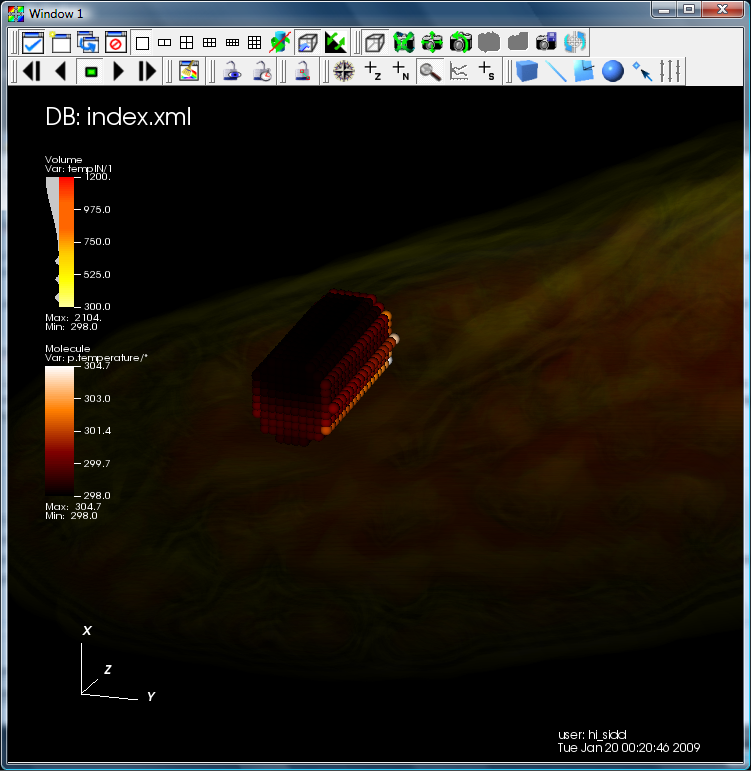
\includegraphics[scale=0.5]{VisItMoleculePTtempViewer.png}
  \caption{Selecting a molecule plot and an associated variable/ material}
  \label{VisItMoleculePTtempViewer}
\end{figure}

\paragraph{Visualizing patch boundaries}
%In order to generate an image, like the one shown in figure~\ref{VisItSubsetPlot}, we use the Subset plot. As with other variables, we select the Subset plot and an associated variable. The variables have a prefix 'level/ patch'. There is a level/ patch variable associated with every kind of variable (Cell Centered, Node Centered, Face Centeerd) present in the dataset. In the figure~\ref{VisItSubsetPlotVariables}, we select one such variable.
In order to visualize patch boundaries, we use the Subset plot. As with other variables, we select the Subset plot and an associated variable. The variables have a prefix 'level/ patch'. There is a level/ patch variable associated with every kind of variable (Cell Centered, Node Centered, Face Centeerd) present in the dataset. In the figure~\ref{VisItSubsetPlotVariables}, we select one such variable.

%\begin{figure}
%  \center
%  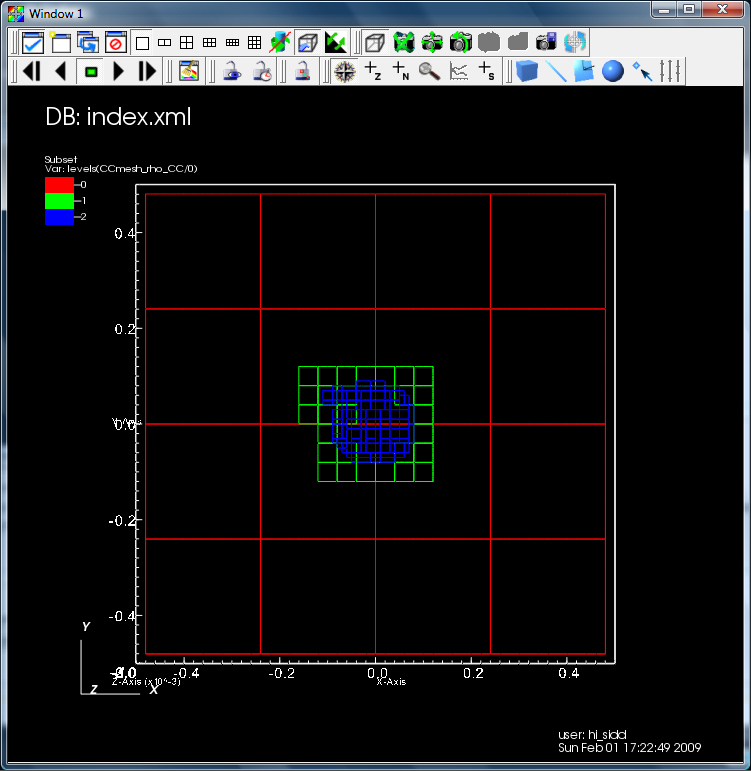
\includegraphics[scale=0.5]{VisItSubsetPlot.png}
%  \caption{Visualizing patch boundaries} 
%  \label{VisItSubsetPlot}
%\end{figure}

\begin{figure}
  \center
  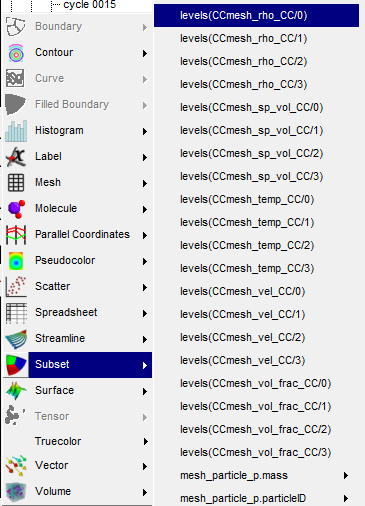
\includegraphics[scale=0.5]{VisItSubsetPlotVariables.png}
  \caption{A patch/ level variable, associated with every kind of variable}
  \label{VisItSubsetPlotVariables}
\end{figure}

Next, we hit Draw. This produces a visualization as shown in figure~\ref{VisItSubsetPlotViewer}. To generate a wireframe model, we double click on the Subset plot in the Active plots window. This pops up the Subset plot attributes window, where we check the Wireframe mode as shown in figure`\ref{VisItSubsetPlotAttrib}. This would produce a visualization, similar to one shown in figure~\ref{VisItSubsetPlotWireframe}.

\begin{figure}
  \center
  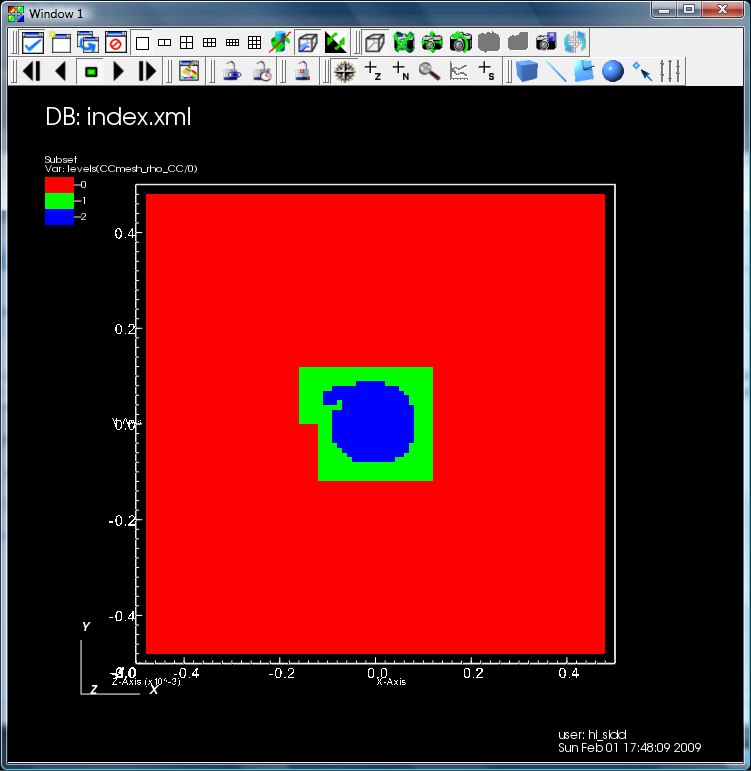
\includegraphics[scale=0.5]{VisItSubsetPlotViewer.png}
  \caption{The default visualization of patches} 
  \label{VisItSubsetPlotViewer}
\end{figure}

\begin{figure}
  \center
  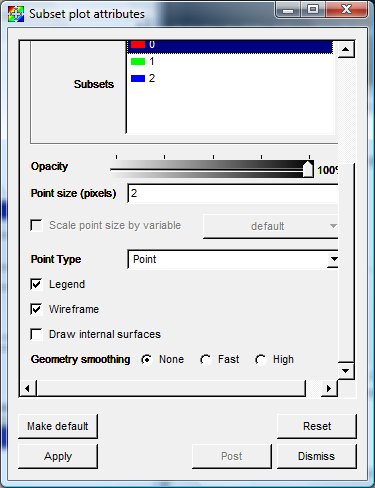
\includegraphics[scale=0.5]{VisItSubsetPlotAttrib.png}
  \caption{Enabling the 'Wireframe' mode for visualizing patch boundaries}
  \label{VisItSubsetPlotAttrib}
\end{figure}

\begin{figure}
  \center
  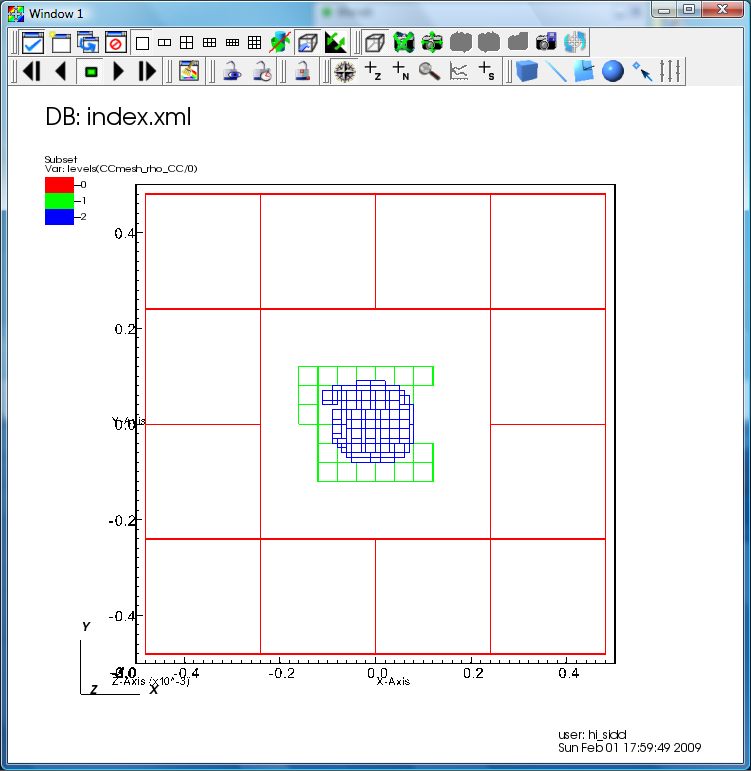
\includegraphics[scale=0.5]{VisItSubsetPlotWireframe.png}
  \caption{The patch boundaries after enabling the wireframe mode}
  \label{VisItSubsetPlotWireframe}
\end{figure}

\subsubsection{Manta}

%__________________________________
\subsection{Data Extraction Tools}

Uintah offers a number of tools for accessing data stored in Uintah Data
Archives (``UDAs").  Because the format of Uintah data is specific to the
framework, these tools allow a user to quickly extract data, which can then
either be postprocessed within that tool (simple modification of the source
code may be necessary), postprocessed with external software such as
Matlab or Octave, or simply plotted with, e.g. gnuplot.  These tools are not compiled automatically when ``make sus'' is issued.  To compile them cd to ``opt/StandAlone/tools'' and issue ``make''.  These tools
are described below.

\subsubsection{puda}

The command line extraction utility \tt puda \normalfont
(for ``parse uintah data archive") has a number of uses.  For example, it
may be used to extract a subset of particle data from a UDA.  Once the
extraction tools have been compiled, the puda executable will be located in 
\tt opt/StandAlone/tools/puda/. \normalfont  If the executable is run with
no additional command line arguments, the following usage information will be
displayed:

\begin{Verbatim}[fontsize=\footnotesize]
Usage: puda [options] <archive file>

Valid options are:
  -h[elp]
  -timesteps
  -gridstats
  -listvariables
  -varsummary
  -jim1
  -jim2
  -partvar <variable name>
  -asci
  -tecplot <variable name>
  -no_extra_cells     (Excludes extra cells when iterating over cells.
                       Default is to include extra cells.)
  -cell_stresses
  -rtdata <output directory>
  -PTvar
  -ptonly             (prints out only the point location
  -patch              (outputs patch id with data)
  -material           (outputs material number with data)
  -NCvar <double | float | point | vector>
  -CCvar <double | float | point | vector>
  -verbose            (prints status of output)
  -timesteplow <int>  (only outputs timestep from int)
  -timestephigh <int> (only outputs timesteps upto int)
  -matl,mat <int>         (only outputs data for matl)
*NOTE* to use -PTvar or -NVvar -rtdata must be used
*NOTE* ptonly, patch, material, timesteplow, timestephigh are used in conjuntion with -PTvar.
\end{Verbatim}

As an example of how to use \tt puda \normalfont, suppose that one wanted to know the locations of all particles at the last archived timestep for the 
\tt const\_test\_hypo.uda \normalfont 
First one may wish to know how many timesteps have been archived.
This could be accomplished by:

\begin{Verbatim}[fontsize=\footnotesize]
 puda -timesteps const_test_hypo.uda
\end{Verbatim}
The resulting terminal output would be:
\begin{Verbatim}[fontsize=\footnotesize]
Parsing const_test_hypo.uda/index.xml
There are 11 timesteps:
1: 1.8257001926347728e-05
548: 1.0012914931998474e-02
1094: 2.0005930425875382e-02
1640: 3.0015616802173569e-02
2184: 4.0005272397960444e-02
2728: 5.0011587657447343e-02
3271: 6.0016178181543284e-02
3812: 7.0000536667661845e-02
4353: 8.0001537138146825e-02
4893: 9.0000702723306208e-02
5433: 1.0001655973087024e-01
\end{Verbatim}

These represent all of the timesteps for which data has been archived.  Suppose now that we wish to know what the stress state is for all particles (in this case two) at the final archived timestep.  For this one could issue:

\begin{Verbatim}[fontsize=\footnotesize]
puda -partvar p.stress -timesteplow 10 -timestephigh 10 const_test_hypo.uda
\end{Verbatim}

The resulting output is:

\begin{Verbatim}[fontsize=\footnotesize]
Parsing const_test_hypo.uda/index.xml
1.00016560e-01 1 0 281474976710656 -2.72031498e-10 -1.05064208e-26 -2.53781271e-08 -1.05064208e-26 -2.72031498e-10 -1.23584688e-09 -2.53781271e-08 -1.23584688e-09 1.63840079e-07
1.00016560e-01 1 1 0 1.93256890e-13 6.56787331e-18 1.85514400e-14 6.56787331e-18 2.24310469e-13 1.85519650e-14 1.85514400e-14 1.85519650e-14 -3.20052991e+06
\end{Verbatim}

The first column is the simulation time, the second column is ????, the third column is the material number, the fourth column is the particle ID, and the remaining nine columns represent the components of the Cauchy stress tensor ($ \sigma_{11}$,$\sigma_{12}$,$\sigma_{13}$, ..., $\sigma_{32}$,$\sigma_{33}$).  If desired, the terminal output can be redirected to a text file for further use.

\subsubsection{partextract}

The command-line utility \tt partextract \normalfont may be used to extract data from an individual particle.  To do this you first need to know the ID number of the particle you are interested in.  This may be done by using the puda utility, or the visualization tools.  Once the extraction tools have been compiled, the partextract utility executable will be located in  \tt /opt/StandAlone/tools/extractors/ \normalfont.  If the executable is run without any arguments the following usage guide will be displayed in the terminal:

\begin{Verbatim}[fontsize=\footnotesize]
No archive file specified
Usage: partextract [options] <archive file>

Valid options are:
  -mat <material id>
  -partvar <variable name>
  -partid <particleid>
  -part_stress [avg or equiv or all]
  -part_strain [avg/true/equiv/all/lagrangian/eulerian]
  -timesteplow [int] (only outputs timestep from int)
  -timestephigh [int] (only outputs timesteps upto int)
\end{Verbatim}

As an example of how to use the partextract utility, suppose we wanted to find the velocity at every archived timestep for the particle with ID 281474976710656 (found above using puda) in the ``const\_test\_hypo.uda'' file (src/StandAlone/inputs/MPM).  The appropriate command to issue is:

\begin{Verbatim}[fontsize=\footnotesize]
partextract -partvar p.velocity -partid 281474976710656 const\_test\_hypo.uda
\end{Verbatim}

The output to the terminal is:

\begin{Verbatim}[fontsize=\footnotesize]
Parsing const_test_hypo.uda/index.xml
1.82570019e-05 1 0 281474976710656 0.00000000e+00 0.00000000e+00 -1.00000000e-02
1.00129149e-02 1 0 281474976710656 -1.03554318e-19 -1.03554318e-19 -1.00000000e-02
2.00059304e-02 1 0 281474976710656 -1.99388121e-19 -1.99388121e-19 -1.00000000e-02
	.
	.
	.
\end{Verbatim}

It is noted that if the stress tensor is output using the partextract utility, the output format is different than for the puda utility.  The partextract utility only outputs the six independent components instead of all nine.  For example, if we use partextract to get the stress tensor for the same particle as above at the last archived timestep only, the output is:

\begin{Verbatim}[fontsize=\footnotesize]
partextract -partvar p.stress -partid 281474976710656 -timesteplow 10 -timestephigh 10 const_test_hypo.uda
Parsing const_test_hypo.uda/index.xml
1.00016560e-01 1 0 281474976710656 -2.72031498e-10 -1.05064208e-26 -2.53781271e-08 -1.05064208e-26 -2.72031498e-10 -1.23584688e-09 -2.53781271e-08 -1.23584688e-09 1.63840079e-07
\end{Verbatim}

Compare this output with the output from puda above.  Notice that the ordering of the six independent components of the stress tensor for partextract are $\sigma_{11}$,$\sigma_{22}$, $\sigma_{33}$, $\sigma_{23}$, $\sigma_{13}$ , $\sigma_{12}$.

\subsubsection{lineextract}

Lineextract is used to extract an array of data from a region of a computational domain. Data can be extracted from a point, along a line, or from a three dimensional region and then stored as a variable for ease of post processing.

Usage: \begin{Verbatim}[fontsize=\footnotesize]
./lineextract [options] -uda <archive file>

Valid options are:
 -h,        --help
 -v,        --variable:      <variable name>
 -m,        --material:      <material number> [defaults to 0]
 -tlow,     --timesteplow:   [int] (sets start output timestep to int) [defaults to 0]
 -thigh,    --timestephigh:  [int] (sets end output timestep to int) [defaults to last timestep]
 -timestep, --timestep:      [int] (only outputs from timestep int) [defaults to 0]
 -istart,   --indexs:        <x> <y> <z> (cell index) [defaults to 0,0,0]
 -iend,     --indexe:        <x> <y> <z> (cell index) [defaults to 0,0,0]
 -l,        --level:         [int] (level index to query range from) [defaults to 0]
 -o,        --out:           <outputfilename> [defaults to stdout]
 -vv,       --verbose:       (prints status of output)
 -q,        --quiet:         (only print data values)
 -cellCoords:                (prints the cell centered coordinates on that level)
 --cellIndexFile:             <filename> (file that contains a list of cell indices)
                                  [int 100, 43, 0]
                                  [int 101, 43, 0]
                                  [int 102, 44, 0]
\end{Verbatim}

The following example shows the usage of lineextract for extracting density data at the 60th computational cell in the x-direction, spanning the width of the domain in the y-direction (0 to 1000), at timestep, 7, (note ``timestep" actually 
refers to the seventh data dump, not necessarily the seventh timestep in the 
simulation. The variable containing the density data within the uda is ``rho\_CC," and the output variable that will store the data for post processing is ``rho."
\begin{Verbatim}[fontsize=\footnotesize]
./lineextract -v rho_CC  -timestep 7 -istart 60 0 0 -iend 60 1000 0 -m 1 -o rho -uda test01.uda.000
\end{Verbatim}

\subsubsection{timeextract}

\subsubsection{compare\_uda}

%__________________________________
\subsubsection{plotting tools}
- plotStats\\
- plotRegridder \\
- plotCPU\_usage \\
- plotComponents

%__________________________________
%FIXME
%\subsection{Code}
%-explain the basic directory structure of src
%\begin{Verbatim}[fontsize=\footnotesize]
%|-- CCA
%|-- Components
%|   |-- Angio
%|   |-- Arches
%|   |-- DataArchiver
%|   |-- Examples
%|   |-- ICE
%|   |-- LoadBalancers
%|   |-- MPM
%|   |-- MPMArches
%|   |-- MPMICE
%|   |-- Models
%|   |-- OnTheFlyAnalysis
%|   |-- Parent
%|   |-- PatchCombiner
%|   |-- ProblemSpecification
%|   |-- Regridder
%|   |-- Schedulers
%|   |-- SimulationController
%|   |-- Solvers
%|   |-- SpatialOps
%|   `-- SwitchingCriteria
%|-- Ports
%|-- Core
%|-- R_Tester
%|-- StandAlone
%|-- Teem
%|-- VisIt
%|-- build_scripts
%|-- include
%|-- orderAccuracy
%|-- scripts
%|-- tau
%|-- testprograms
%`-- tools
%\end{Verbatim}
